\section{Kürzeste Wege Probleme}
\begin{definition}[gewichteter Graph]
Sei $G=(V,E)$ ein Graph. Eine \emph{Gewichtsfunktion} für die Kanten von $G$ ist eine Abbildung $w \colon E \to R$. Ist $\pi=v_0,v_1,\ldots,v_r$ ein Weg, so heißt
\[
w(\pi) = \sum_{i=1}^{r-1}w(v_i,v_{i+1})
\]
die \emph{Weglänge} von $\pi$ bezüglich $w$. Das Tripple $G=(V,E,w)$ heißt \emph{gewichteter Graph}. 
\end{definition}
\begin{definition}
	\label{def:negative_gewichte}
Sei $G=(V,E,w)$  ein gewichteter Graph und $v, \tilde{w} \in  V$. Ein \emph{kürzester Weg} von $v$ nach $\tilde{w}$  in $G$  bezüglich $w$ ist ein $v\text{-} \tilde{w}$-Weg $\pi$  mit der Eigenschaft $w(\pi) \le w(\pi')$  für alle anderen $v\text{-}w$-Wege $\pi'$ .
Die kürzeste Weglänge $\delta(v,\tilde{w})$  von $v$ nach $\tilde{w}$ ist definiert durch:

\begin{center}$\delta(v,\tilde{w}) \begin{cases}
	\min \{w(\pi) | \pi \text{ ist $v$-$\tilde{w}$-Weg  }\} &, \text{falls ein solcher Weg existiert} \\
	\infty &, \text{ sonst}
\end{cases}$ \end{center}
\end{definition}

\begin{example}
Betrachte den gewichteten Graph $G=(V,E,w)$ mit

\begin{center}
\begin{tikzpicture}

%Nicer Graph


\end{tikzpicture}
\end{center}
Mögliche Wege von $v_3$ nach $v_1$ sind:
\begin{align*}
	\pi_1&=v_3,v_1 &\implies w(\pi_1)&=6 \\
	\pi_2&=v_3,v_2,v_1 &\implies w(\pi_2)&=5 \\
	\pi_3&=v_3,v_4,v_2,v_1 &\implies w(\pi_3)&=9
\end{align*}
\end{example}
\begin{notation}
Wir werden im Folgenden nur Digraphen behandeln, da sich ungerichtete Graphen immer auch als gerichtete Graphen interpretieren lassen.
Sei $G=(V,E,w) $ ein gewichteter Digraph.
\end{notation}
Wir unterscheiden drei verschiedene Varianten des \emph{kürzeste-Wege-Problems:}
\begin{enumerate}
	\item Einzelpaar-kürzeste-Wege-Problem \\
		Gegeben $v,u \in V$ , suche einen kürzesten Weg von v nach u.
	\item Einzelquelle-kürzeste-Wege-Problem \\
		Gegeben $v \in V$, suche einen kürzesten Weg von $v$ zu allen $u \in post^{*}(v)$.  
	\item Alle-Paare-kürzeste-Wege-Problem \\
		Finde alle Paare $v,u \in V$ einen kürzesten $v$-$u$-Weg
\end{enumerate}
Wir bemerken, dass das Problem c die Probleme a und b löst, daher betrachten wir im Folgenden nur Problem c. \\
Negative Gewichte sind zwar nach Definition \ref{def:negative_gewichte} zugelassen, können aber Probleme bereiten:
\begin{example}
Betrachte:
\begin{center}
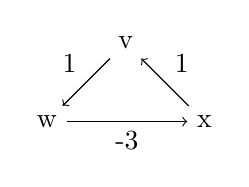
\begin{tikzpicture}
 \node (v) at (0,0) {v};
 \node (w) at (-1,-1) {w};
 \node (x) at (1,-1) {x};

 \path [->] (v) edge node[above left] {1} (w);
 \path [->] (w) edge node[below] {-3} (x);
 \path [->] (x) edge node[above right] {1} (v);
\end{tikzpicture}
\end{center}
In diesem Graphen gibt es keinen kürzesten Weg.
\begin{align*}
	w(v,w,x)&=-2 \\
	w(v,w,x,v,w,x)&=-3
\end{align*}
Man kann den Weg also immer weiter verlängern und der Weg wird immer kürzer.
\end{example}
\begin{lemma}
	Sei $G=(V,E,w)$  ein gewichteter Digraph. Falls es in $G$ keine Zyklen mit negativer Weglänge gibt, dann gibt es für $v,u \in V, u \in  post^{*}(v)$ einen kürzesten Weg $\pi$ mit:
	\[
	\delta(v,w) = w(\pi) > -\infty
	\]
\end{lemma}
\begin{proof}
Da es keine negativen Zyklen gibt, genügt es alle einfachen Wege von $v$ nach $u$ zu betrachten. Da $|V|$ und $|E|$ endlich sind, sind dies endlich viele, so dass $\pi$ durch einen Minimierer gegeben ist.
\end{proof}

\begin{lemma}
	\label{lem:teilweg}
	Sei $G=(V,E,w)$ ein gewichteter Digraph ohne negativen Zyklen. Ist $\pi= v_0, \ldots, v_r$ ein kürzester Weg von $v_0$  nach $v_r$ dann ist der Teilweg
	\[
		\pi_{i,j} =v_i,\ldots,v_j, 0\le i  <j \le r
	\]
ein kürzester Weg von $v_i$ nach $v_j$.
\end{lemma}
\begin{proof}
\underline{Angenommen:} $\pi_{i,j}'$ ist ein kürzester Weg von $v_i$ nach $v_j$ mit $w(\pi_{i,j}'  < w (\pi_{i,j})$
\begin{align*}
	\implies \pi' &= \pi_{0,i} \pi_{i,j}' \pi_{j,r} \text{ erfüllt:}\\
	w(\pi')&= w(\pi_{0,i})+w(\pi_{i,j}')+w(\pi_{j,r}) \\
	       &< w(\pi_{0,i})+ w(\pi_{i,j}) + w(\pi_{j,r})\\
	       &= w(\pi') \\
	       &\implies w(\pi') < w(\pi)
\end{align*}
Dies ist ein Widerspruch, da $\pi$ kürzester Weg nach Annahme ist.
\end{proof}
\begin{lemma}
	\label{lem:delta_delta_w}
	Sei $G=(V,E,w)$ ein gewichteter Digraph ohne negative Zyklen und sei $\pi=v_0,v_1,\ldots,v_r$ ein kürzester Weg von $v_0$ nach $v_r$ . Dann gilt:
	\[
	\delta(v_0,v_r)= \delta(v_0, v_{r-1} + w(v_{r-1}, v_r)
	\]
\end{lemma}
\begin{proof}
Aus Lemma \ref{lem:teilweg} folgt:
\begin{itemize}
	\item $\pi' = v_0,\ldots, v_{r-1}$ ist ein kürzester Weg von $v_0$ nach $v_{r-1}$
	\item $\delta(v_0,v_{r-1} = w(\pi')$
	\item $\delta(v_0,v_r)= w(\pi)$	
\end{itemize}
$w(\pi)$ lässt sich umschreiben:
\begin{align*}
	w(\pi)&= w(\pi')+w(v_{r-1},v_r) \\
	      &= \delta(v_0,v_{r-1} + w(v_{r-1},v_r)
\end{align*}
\end{proof}

\begin{algorithm}[H]
	\label{alg:dijkstra}
	\caption{Dijkstra Algorithmus}
	\KwData{Gewichteter Graph $G=(V,E,w)$ mit nicht negativen Gewichten}
	\KwResult{Kürzeste Wege von $s$ nach $v \in post^{*}(s)$ samt Weglänge $l(v)=\delta(s,v)$}
\begin{itemize}
	\item $l(s)=0$ \\$l(v) = \infty$, $v \in V \setminus \{s\} $ \\$R=\emptyset$ 
	\item Finde $u \in V\setminus R$ mit $l(n)= \min_{v \in V \setminus R} l(v)$
	\item $R=R \cup \{u\} $ 
	\item \For{$v \in V \setminus R$ mit $(u,v) \in E$}{
			\If{$l(v)> l(u)+w(u,v)$}{
				$l(v) = l(u)+w(u,v)$\\
				$p(v)=u$ }}
	\item $R \neq  V $ gehe zu 2. 
\end{itemize}
\end{algorithm}
\begin{remark}
Die kürzesten Wege im Output des Algorithmus sind durch die Abbildung $p \colon V \to V $ gegeben, denn
\[
	\pi=s,\ldots, p(p(p(v))),p(p(v)),p(v),v
\]
ist ein kürzester $s$-$v$-Weg.
\end{remark}
\begin{example}
Der Graph
\begin{center}
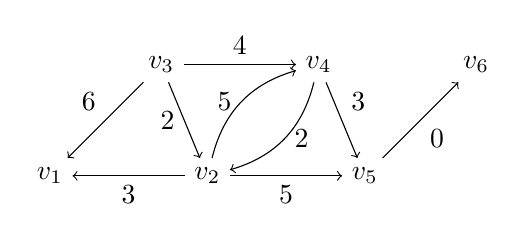
\begin{tikzpicture}[node distance = 2cm, auto]

	\node (v3) {$v_3$};
	\node (v4) [right of=v3] {$v_4$};
	\node (v1) [below left of=v3] {$v_1$};
	\node (v2) [right of=v1] {$v_2$};
	\node (v5) [right of=v2] {$v_5$};
	\node (v6) [above right of=v5] {$v_6$};

	\path[->] (v5) edge node[below right] {0} (v6);
	\path[->] (v2) edge node[below] {5} (v5);
	\path[->] (v2) edge node[below] {3} (v1);
	\path[->] (v4) edge node[above right]{3} (v5);
	\path[->] (v3) edge node[above left] {6} (v1);
	\path[->] (v3) edge node[above] {4} (v4);
	\path[->] (v4) edge[bend right=-30] node[right] {2} (v2);
	\path[->] (v2) edge[bend left=30] node[left] {5} (v4);
	\path[->] (v3) edge node[left] {2} (v2);
		
\end{tikzpicture}
\end{center}
mit Startknoten $v_3$ hat nach Ausführung von Algorithmus \ref{alg:dijkstra} folgende Ausgabe:
\clearpage
\begin{table}[htbp]
	\centering\renewcommand{\arraystretch}{1.2}
	\caption{Dijkstra}
	\label{tab:dijkstra}
	\begin{tabular}{c|c c c c c c| c c c}
Iteration & \multicolumn{6}{c|}{$l(v_1),l(v_2),\ldots,l(v_6)$} & \multicolumn{3}{c}{$u$, $l(u)$, $p(u)$  } \\
\hline
$0$ & $\infty$ & $\infty$ & $0$ & $\infty$ & $\infty$ & $\infty$ & $v_3$ & $0$ &$-$ \\     
$1$ & $6$ & $2$ & & $4$ & $\infty$ & $\infty$ & $v_2$ & $2$ & $v_3$ \\
$2$ & $5$  & & & &  $7$ & $\infty$ & $v_4$ & $4$ & $v_3$  \\
$3$ & & & & & & $\infty$ & $v_1$ & $5$ & $v_2$ \\
$4$ & & & & & & $\infty$ & $v_5$ & $7$ & $v_2$ \\
$5$ & & & & & & $7$ & $v_6$ & $7$ & $v_5$ \\
	\end{tabular}
\end{table}
\end{example}
\begin{theorem}
Der Algorithmus von Dijkstra \ref{alg:dijkstra} arbeitet korrekt, mit einer Laufzeit von $\mathcal{O}(n^2), n=|V|$.
\end{theorem}
\begin{proof}
\begin{notation}
Schreibe in der k-ten Iteration $^{(k)}$ an alle Größen, die im Algorithmus vorkommen
\end{notation}
\underline{Zeige:} Bei jeder Ausführung von 2. gilt:
\begin{enumerate}
	\item $l^{(k)}(v) \le l^{(k)}(y)$ für alle $v \in R^{(k)}, y \in V \setminus R^{(k)}$
	\item $l^{(k)}(v)=\delta(s,v)$ für alle $v \in R^{(k)}$ \\
	$l^{(k)}(v)<\infty, v \neq s \implies$ Es existiert ein kürzester s-v-Weg mit Knoten in $R^{(k)}$ und letzter Kante $(p(v),v)$
\item $v \in V \setminus R^{(k)} \implies l^{(k)}(v)$ ist die kürzeste Weglänge 
	von s nach v im Teilgraphen mit Knoten $R^{\left( k \right)} \cup \{v\} $ in $G$ \\
	$v \in V \setminus R^{(k)}, l^{(k)}(v)<\infty \implies p^{(k)}(v) \in R^{(k)}$ und $l^{(k)}(v)=l^{(k)}(p(v))+w(p^{(k)}(v),v)$  
\end{enumerate}
Per vollständiger Induktion:

\begin{itemize}[label=$\lozenge$, itemsep=2ex]
	\item IV \underline{$k=0$} Trivialerweise erfüllt
	\item IS \underline{$k \to k+1$} Sei u der in 2. ausgewählte Knoten.
		\paragraph{a)} Für $v \in R^{(k)}, y \in V \setminus R^{(k)}$ gilt:
		\begin{align*}
			l^{(k+1)}(v)&= l^{(k)}(v) \\
				    &\le  l^{(k)}(u) \\
				    &= \min_{u \in V \setminus R^{(k)}} l^{(k)}(u)\\
				    &\le l^{(k+1)}(y)
		\end{align*}
Da $R^{(k+1)}=R^{(k)}\cup \{u\} \implies $ Behauptung a) für $k+1$ gilt.

\paragraph{b)} Wir müssen die Behauptung über die kürzeste Weglänge nur für u überprüfen.\\

c) für $k \implies l^{(k)}(u)$ ist die kürzeste Weglänge zum Weg $\pi$ im Teilgraphen $R^{(k)}\cup \{u\}$. \\
\underline{zu Zeigen} $l^{(k+1)}(u)=l^{(k)}(u)=w(\pi) = \delta(s,u)$ in $G$ \\
\underline{Angenommen:} Es gibt einen Weg $\pi'$ in $G$ mit mindestens einem Knoten $y \in V \setminus R^{(k)}$ und $w(\pi' < w(\pi)$ \\
$\pi' = s,v_1,\ldots,v_{r-1},y,v_{r+1},\ldots,v_{r+m},u$ \\
\begin{align*}
	\implies l^{(k)}(y) &\le  w(s,v_1,\ldots,v_{r-1},y) \\
			    &\le w(\pi') \\
			    &< w (\pi) \\
			    &= l^{(k)}(u)
\end{align*}
Dies ist ein Widerspruch zu $l^{(k)}(u)= \min_{v \in V \setminus R^{(k)}} l^{(k)}(v)$ \\
$\implies b$ für $k+1$
\end{itemize}
\paragraph{c)}
Zeige, dass 3. und 4. die Aussage c) erhalten. Sei $v \in V \setminus R^{(k+1)}$ in 4. \\
\begin{align*}
	\implies p^{(k+1)}(v)&= u \\
	l^{(k+1)}(v) &= l^{\left( k+1 \right)}(u) +w(u,v)
\end{align*}
c) für $k \implies $ Es gibt einen s-v-Weg im von $R^{(k+1)}\cup \{v\} $ aufgespannten Teilgraph $G'(v)$  in $G$ , mit Länge $l^{(k+1)}(v)= l^{(k+1)}(u)+w(u,v)$ \\
\underline{zu Zeigen} Dieser Weg ist ein kürzester Weg in $G$ \\
\underline{Angenommen:} Für ein $v \in V \setminus R^{(k+1)}$ in 4. gibt es einen s-v-Weg $\pi$ in $G'(v)$ mit $w(\pi) < l^{(k+1)}(v)$. \\
Beobachte: $l^{(k+1)}(v) \le l^{(k)}(v)$ \\
$\implies u$ muss $\pi$ enthalten sein, da dies die einzige Veränderung zum k-ten Schritt ist und $l^{(k)}(v)$ nach c) im k-ten Schritt ein kürzester Weg in $R^{(k)}\cup \{u\} $ ist. \\
Sei $x$ der Vorgänger von $v$  in $\pi$. 
\begin{align*}
	l^{(k+1)}(v)&= l^{(k+1)}(x) + w(x,v) \\
		    &\le l^{(k+1)}(u) + w(x,u) \\
		    &\le w(\pi)
\end{align*}
Dies ist ein Widerspruch $\implies $ c) für $k+1$. Für $k=n$ impliziert b) die Behauptung. 
\paragraph{Aufwand:} $\mathcal{O}(n^2)$ ist trivial. 
\end{proof}
\begin{remark}
Clevere Implementierungen können den Dijkstra-Algorithmus \ref{alg:dijkstra} in $\mathcal{O} (m+n\log(n), n=|V|, m=|E|$ durchführen.
\end{remark}
Für die Verallgemeinerung für negative Gewichte betrachten wir folgend den Moore-Bellmann-Ford Algorithmus: \\
\begin{algorithm}[H]
	\label{alg:mbf}
	\caption{Moore-Bellmann-Ford}
	\KwData{Gewichteter Digraph $G=(V,E,w)$ ohne negative Zyklen, Startknoten $s \in V$ }
	\KwResult{kürzeste Wege von s nach v, $v \in post^{*}(s)$ samt Weglänge $l(v)=\delta(s,v)$} 
\begin{itemize}
	\item $l(s)=0$\\
	$l(v)=\infty, v \in V \setminus \{s\}$ 
\item \For{$k = 1,...,n-1$}{\For{$e =(u,v) \in  E$}{\If{$l(v)>l(u)+w(u,v)$}{$l(v)=l(u)+w(u,v)$\\ $p(v)=u$}   }}
\end{itemize}
\end{algorithm}
\begin{example}
Betrachte den Graphen:
\begin{center}
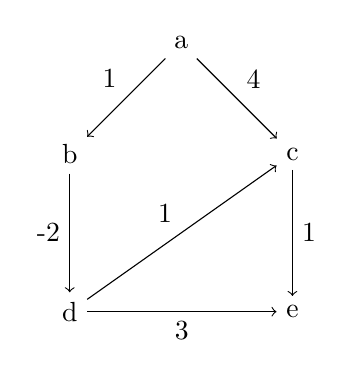
\begin{tikzpicture}[node distance = 2cm, auto]
\node (q) {a};
\node (b) [below left of=q] {b};
\node (c) [below right of=q] {c};
\node (d) [below of=b] {d};
\node (e) [below of=c] {e};

\path [->] (q) edge node[above left] {1} (b);
\path [->] (q) edge node[above right] {4} (c);
\path [->] (b) edge node[left] {-2} (d);
\path [->] (c) edge node[right] {1} (e);
\path [->] (d) edge node[above left] {1} (c);
\path [->] (d) edge node[below] {3} (e);
\end{tikzpicture}
\end{center}
mit Startknoten a.
\clearpage
\begin{table}[htpb]
	\centering
	\caption{Iteration 1}
	\label{tab:bmf-1}
	\begin{tabular}{c| c c c c c|c c c c}
		Kante & \multicolumn{5}{c|}{$l(a) , \ldots, l(e)$} & \multicolumn{4}{|c}{$p(b),\ldots,p(e)$} \\ 
		\hline
		$(a,b)$ & 0 & 1 & $\infty$ & $\infty$ & $\infty$  & a & - & - & - \\
		$(a,c)$ & & & 4 & $\infty$ & $\infty$  & & a & - & - \\
		$(b,d)$ & & & 4 & $-1$ & $\infty$ & & a & & c \\ 
		$(c,e)$ & & & 4 & &5 & & a & &c \\
		$(d,c)$ & & & 0 & & 5 & & d & &c \\
		$(d,e)$ & & & & & 2 & & & & d

		 
	\end{tabular}
\end{table}
\begin{table}[htpb]
	\centering
	\caption{Iteration 2}
	\label{tab:bmf-2}
	\begin{tabular}{c| c c c c c|c c c c}
		Kante & \multicolumn{5}{c|}{$l(a),\ldots,l(e)$} & \multicolumn{4}{|c}{$p(b),\ldots, p(e)$}\\
		\hline
		$(a,b)$ & $0$ & $1$ & $0$ & $-1$ & $2$ & a & d & b & d \\
		$(a,c)$\\
		$(b,d)$ \\
		$(c,e)$ \\
		$(d,c)$ & & & & & $1$ & & & & c \\
		$(d,e)$ 


	\end{tabular}
\end{table}
Keine Veränderung mehr ab der 3. Iteration.
\end{example}

\begin{theorem}
	Der Moore-Bellman-Ford Algorithmus \ref{alg:mbf} arbeitet korrekt mit Aufwand $\mathcal{O}(m \cdot n), m =|E|, n=|V|$. 
\end{theorem}
\begin{proof} 
Bezeichne zu jedem Zeitpunkt:
\begin{align*}
	R &= \{v \in V | l(v) < \infty\} \\
	F &= \{(u,v) \in E | u = p(v)\} 
\end{align*}
Zeige zu erst:
\begin{enumerate}
	\item $l(v) \ge l(u) + w(u,v), (u,v) \in E$ 
	\item $(R,F)$  ist ein azyklischer Graph
	\item $(R,F)$ ist ein gerichteter Baum mit Wurzel $s$, d.h jeder Knoten in $R$ ist über genaue einen Weg von $s$ aus erreichbar.
\end{enumerate}
\paragraph{a)} Bei $p(v)=u$ gilt:
\[
l(v)=l(u)+w(u,v)
\]
Danach wird $l(u)$ höchstens verkleinert.
\paragraph{b)}
\underline{Angenommen:} Es gibt einen Zyklus $\pi=v_0,v_1,\ldots,v_{r-1},v_r$ mit $v_0=v_r$ \\
Ohne Beschränkung der Allgemeinheit entstanden durch Setzen von $p(v_r)=v_{r-1}$ \\
$\implies$ Davor galt:
\[
l(v_0)=l(v_r) > l(v_{r-1}) + w(v_{r-1},v_r)
\]
Wegen a) gilt:
\[
l(v_{i+1}) \ge l(v_i) +w(v_i, v_{i+1}, i=0,\ldots,r-2)
\]
\begin{align*}
	\implies \sum_{i=1}^{r}w(v_{i-1},v_i) &= \left( \sum_{i=1}^{r-1}w(v_{i-1},v_i) \right)+ w(v_{r-1},v_r) \\
					      &< \sum_{i=1}^{r}(l(v_i)-l(v_{i-1}) \\
					      &=0
\end{align*}
Widerspruch dazu, dass es keine negativen Zyklen gibt.

\paragraph{c)}
$x \in R \setminus \{s\} \implies p(x)=R$ Gehe von Blättern zu Wurzel dann folgt c)\\
$a,b,c \implies l(y)$ ist mindestens die Länge des (eindeutigen) s-y-Wegs in $(R,F)$ \\
\underline{Behauptung:} Nach k Iterationen ist $l(y)$ auch die maximale Länge eines kürzesten s-y-Wegs in $G$ mit maximal k Kanten.\\
Zeige durch Induktion:
\begin{itemize}[label=$\lozenge$, itemsep=2ex]

	\item IV \underline{$k=1$} klar
	\item \underline{$k-1 \to k$} Sei 
		\[
		\pi=s,v_1,\ldots,v_r,x,y
		\]
	ein kürzester s-y-Weg in G mit höchsten k Kanten und $r\le k-2$. \\
	Dann folgt aus Lemma \ref{lem:delta_delta_w}:
	\begin{itemize}
		\item $\pi'=s,v_1,\ldots,v_r,x$ ist ein kürzester s-k-Weg mit k-1 Kanten
		\item $l(x)\le w(\pi')$
		\item \begin{align*}
				l(y)&\le l(x)+w(x,y) \\
				    &\le w(\pi') + w(x,y) \\
				    &= w(\pi)
		\end{align*}
	\end{itemize}
\end{itemize}
Wir haben gezeigt: $w(\pi) = \delta(s,y)$, wobei $\pi$ der eindeutige Weg in $(R,T)$ mit maximal k Kanten. \\
Daraus folgt die Behauptung.
\paragraph{Aufwand:} Trivial.
\end{proof}
Die letzte Frage dieses Kapitels: Algorithmus für das Alle-Paare-kürzeste-Wege Problem lässt eine naive Antwort zu. Diese lautet: Wende Dijkstra oder Moore-Belmann-Ford auf jede Quelle an.Das Resultat ist jedoch, dass man keine brauchbaren Datenstrukturen mehr hat. Demnach gibt es folgenden Algorithmus:\\
Ohne Beschränkung der Allgemeinheit sei $V=\{1,\ldots,n\} $ \\
\begin{algorithm}[H]
	\label{alg:fw}
	\caption{Floyd-Warshall}
	\KwData{Gewichteter Digraph $G=(V,E,w), V=\{1,\ldots,n\} $ ohne negative Zyklen}
	\KwResult{Matrizen $[l_{i,j}]_{i,j=1}^{n}, [p_{i,j}]_{i,j=1}^{n}$}
	\begin{itemize}
		\item \begin{align*}
				l_{i,j} &= w(i,j) &,(i,j) \in E \\
				l_{i,j} &= \infty &,\forall (i,j) \in (V\times V)\backslash E, i = j\\
				l_{i,i} = 0 &, i \in V \\
				p_{i,j} &= i &, i,j \in V
		\end{align*}
		\item \For{$j = 1,...,n$}{\For{$i = 1,...,n, i\neq j$}{\For{$k = 1,...,n, k \neq j$}{
			\If{$l_{i,k} > l_{i,j} + l_{j,k}$}
			{
				$l_{i,k} = l_{i,j} + l_{j,k}$
				$p_{i,k} = p_{j,k}$
			}
		}}}
\end{itemize}
\end{algorithm}
\begin{theorem}
	Der Algorithmus \ref{alg:fw} arbeitet korrekt, mit Aufwand $\mathcal{O}(n^3), n=|V|$ 
\end{theorem}
\begin{proof}
\begin{notation}
Im Iterationsschritt $j_0$ ist $l_{ik}^{(j_0)}$ die Länge eines kürzesten i-k-Weges im von $\{1,\ldots,j_0\} $ aufgespannten Teilgraphen mit Endkante $(p_{ik}^{(j_0)},k)$. 
\end{notation}
\end{proof}
